% Manual de usuario: lo usan documentacion.tex (anexo) y manual_usuario.tex (aparte)
\manualseccion{Instalación}

\ggez\ se entrega como un único archivo ejecutable, generado con \kw{publicar.sh}. No requiere instalar .NET ni Python.

\begin{itemize}
  \item \textbf{Linux}: dar permiso de ejecución y abrirlo: \kw{chmod +x GGEZ} y luego \kw{./GGEZ}.
  \item \textbf{Windows}: abrir \kw{GGEZ.exe}.
\end{itemize}

La primera vez, el IDE despliega el traductor y su Python en la carpeta de datos del usuario; esto toma unos segundos y no se repite. Para generar el ejecutable desde el código fuente: \kw{./publicar.sh linux}, \kw{./publicar.sh windows} o \kw{./publicar.sh todo}; el resultado queda en la carpeta \kw{dist/}.

\manualseccion{La ventana principal}

\begin{figure}[H]
\centering
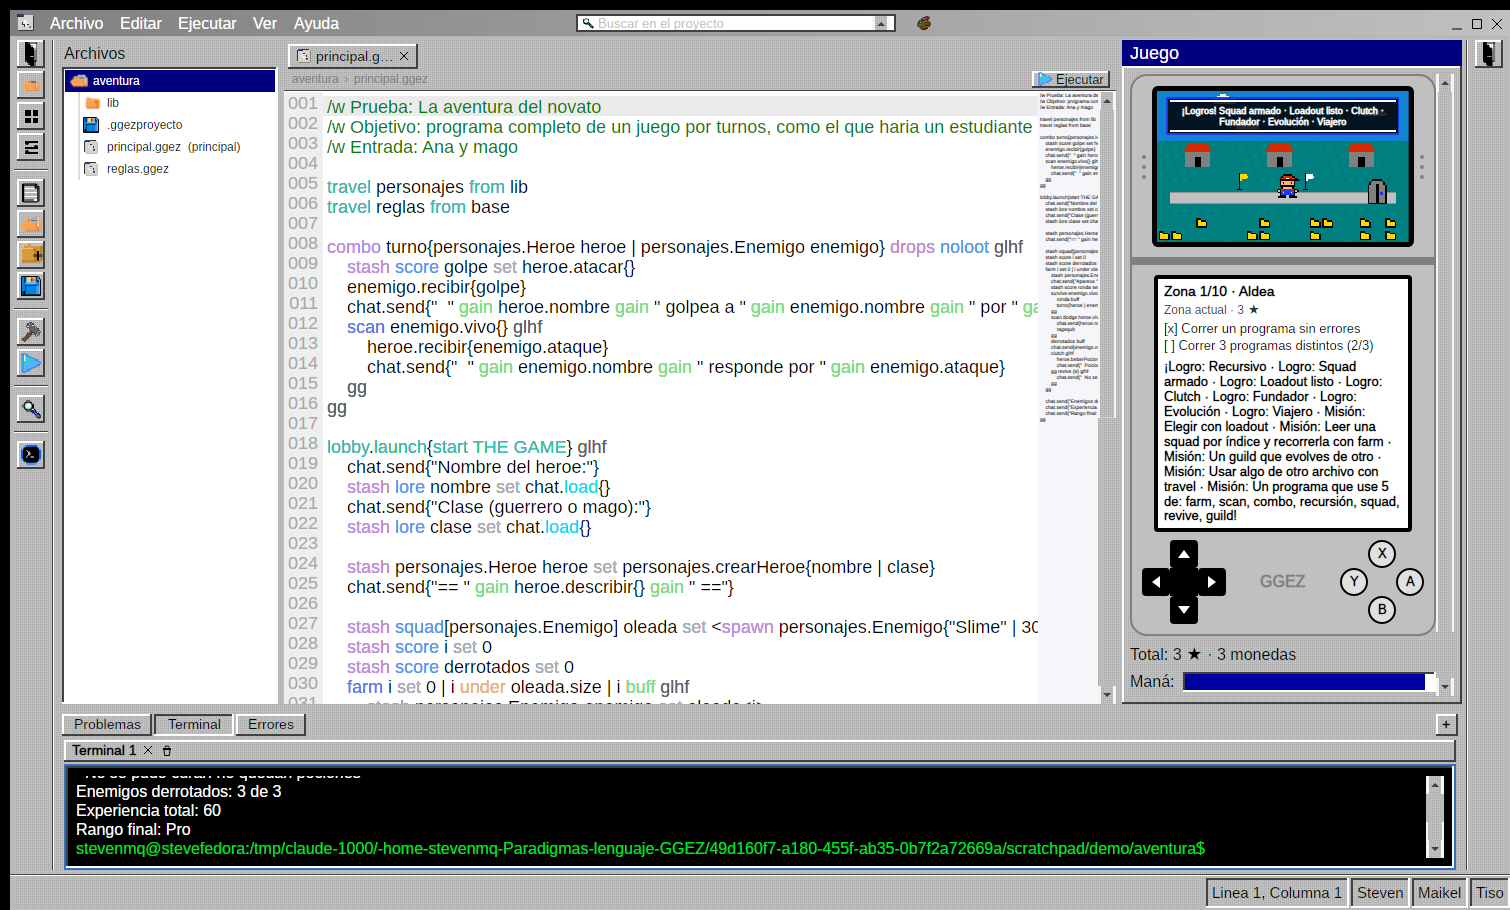
\includegraphics[width=\textwidth]{img/ide_ejecucion.png}
\caption{Ventana principal del IDE.}
\end{figure}

\begin{itemize}
  \item \textbf{Barra de menú} (arriba): Archivo, Editar, Ejecutar, Ver y Ayuda.
  \item \textbf{Barra lateral} (izquierda): íconos para cambiar entre el explorador de archivos, las extensiones y los ajustes.
  \item \textbf{Explorador}: el árbol de archivos del proyecto abierto.
  \item \textbf{Editor} (centro): pestañas con los archivos abiertos, números de línea, coloreado de sintaxis y minimapa a la derecha. Sobre el editor están la ruta del archivo y los botones de compilar (martillo) y ejecutar (reproducir).
  \item \textbf{Segmento de salida} (abajo): pestañas Terminal, Errores y Problemas.
  \item \textbf{Panel de juego} (derecha): maná, mapa del mundo, nivel actual, monedas, pistas y logros.
  \item \textbf{Barra de estado} (abajo del todo): línea y columna del cursor y otros datos.
\end{itemize}

El tamaño del explorador, del panel de juego y de la terminal se cambia arrastrando el divisor que los separa del editor; el divisor se resalta al pasar el mouse.

\manualseccion{Crear y abrir un proyecto}

\begin{enumerate}
  \item Menú \textbf{Archivo → Abrir carpeta} (\kw{Ctrl+O}) y elegir o crear una carpeta.
  \item En el explorador, clic derecho para crear archivos (\kw{.ggez}) y carpetas, renombrar o eliminar. Los archivos y carpetas que se crean, borran o editan fuera del IDE aparecen solos en el árbol, y una pestaña abierta sin cambios sin guardar se recarga con el contenido nuevo.
  \item Opcional: clic derecho sobre un archivo con \kw{lobby.launch} → \textbf{Marcar como principal}. El archivo aparece con la etiqueta «(principal)» y se usa cuando la pestaña enfocada no es un \kw{.ggez}.
\end{enumerate}

Sin proyecto abierto, también se puede crear un archivo suelto con \kw{Ctrl+N}, guardarlo y ejecutarlo.

\manualseccion{Escribir código}

\begin{itemize}
  \item El editor colorea palabras reservadas, tipos, operadores, textos y comentarios.
  \item \textbf{Autocompletado}: aparece al escribir o con \kw{Ctrl+Espacio}. Sugiere palabras reservadas, plantillas completas (por ejemplo, un \kw{farm} con sus tres partes) con su descripción, los nombres declarados en el archivo y, después de un punto, los miembros disponibles (\kw{chat.send}, \kw{lista.recruit}, lo de un módulo importado). Con las flechas se elige y con \kw{Enter} o \kw{Tab} se inserta; \kw{Esc} cierra la lista.
  \item \textbf{Minimapa}: muestra todo el archivo en miniatura a la derecha del editor; un clic salta a esa parte.
  \item Con la extensión de colores de bloques, al presionar \kw{Enter} después de \kw{glhf} el editor cierra el bloque con \kw{gg}.
  \item \kw{Ctrl+F} busca, \kw{Ctrl+H} reemplaza y \kw{Ctrl+G} va a una línea.
\end{itemize}

\begin{figure}[H]
\centering
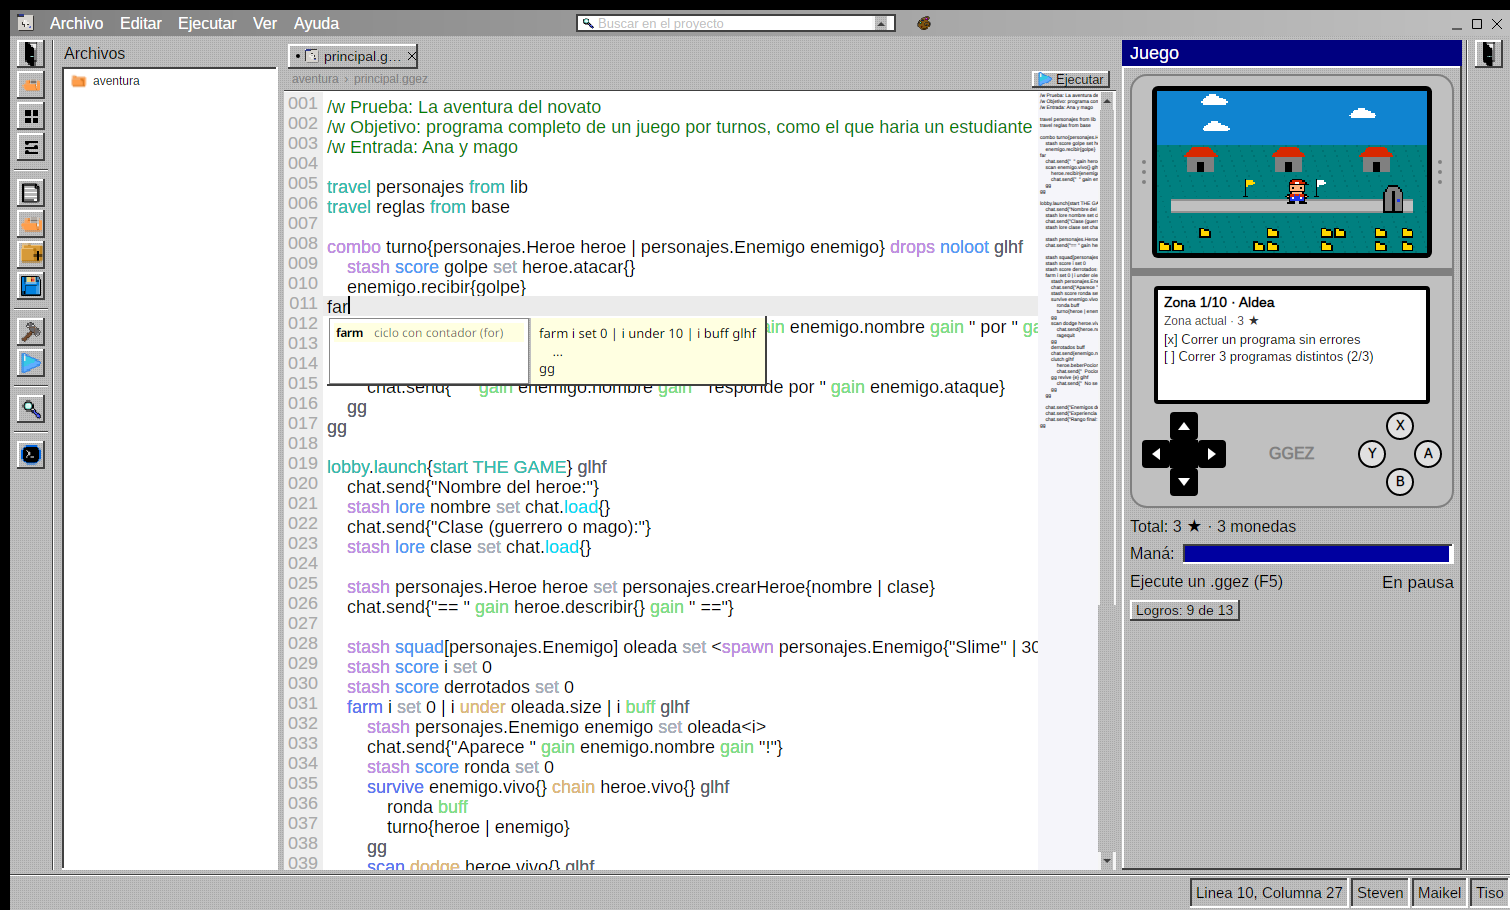
\includegraphics[width=0.92\textwidth]{img/autocompletado.png}
\caption{Autocompletado con plantillas y su descripción.}
\end{figure}

\manualseccion{Compilar y ejecutar}

\begin{itemize}
  \item \textbf{Compilar} (\kw{F6} o el martillo): revisa el archivo \kw{.ggez} de la pestaña enfocada sin ejecutarlo. Si todo está bien, la terminal muestra «Compilacion exitosa».
  \item \textbf{Ejecutar} (\kw{F5} o el botón de reproducir): compila y, si no hay errores, ejecuta el archivo \kw{.ggez} de la pestaña enfocada. Lo que imprime el programa aparece en celeste. Cuando el programa pide datos con \kw{chat.load}, se escriben en la terminal y se presiona \kw{Enter}.
  \item \kw{Ctrl+C} en la terminal detiene un programa en ejecución.
\end{itemize}

\manualseccion{Corregir errores}

\begin{enumerate}
  \item Si hay un error, la terminal lo muestra en rojo y la pestaña \textbf{Problemas} lo lista con su tipo, archivo, línea y posible causa.
  \item Un clic sobre el problema abre el archivo y lleva el cursor a la línea.
  \item Las advertencias aparecen en amarillo y no impiden ejecutar.
  \item Menú \textbf{Ejecutar → Ver errores} abre la pestaña de errores.
\end{enumerate}

\manualseccion{Terminal}

La terminal permite escribir comandos del sistema y tiene comandos propios: \kw{cd}, \kw{clear}, \kw{exit} y \kw{help}. Con el botón \textbf{+} se abren hasta cuatro terminales, una al lado de la otra. La primera terminal es siempre la terminal de \ggez, donde se compila y ejecuta. Con la extensión de Claude instalada, al escribir \kw{claude} en ella se abre otra terminal al lado con el asistente; en sus menús se elige con las flechas y \kw{Enter}.

Colores de la terminal: verde el indicador, blanco lo que escribe el usuario, celeste la salida del programa, rojo los errores y amarillo los avisos y advertencias.

\manualseccion{Modo de juego}

\begin{itemize}
  \item \textbf{Maná}: la barra muestra cuánto gastó el último programa.
  \item \textbf{Mapa}: muestra la zona actual y sus misiones; las flechas recorren las zonas. Al cumplir todas las misiones de una zona se abre la siguiente.
  \item \textbf{Niveles}: abrir la carpeta de un nivel (con \kw{nivel.json}) y ejecutar el archivo; el panel muestra cuántas pruebas pasaron y las estrellas ganadas.
  \item \textbf{Pistas}: el botón de pista gasta una moneda y muestra la siguiente pista del nivel.
  \item \textbf{Logros}: la lista muestra los obtenidos y los pendientes.
\end{itemize}

\manualseccion{Extensiones y ajustes}

En la vista de \textbf{Extensiones} se instalan y desinstalan complementos con un clic, entre ellos los temas desbloqueados con estrellas. En \textbf{Ajustes} se cambian el tamaño de letra, el zoom y otras preferencias del editor. Todo se conserva al cerrar el IDE, junto con las pestañas abiertas.

\begin{figure}[H]
\centering
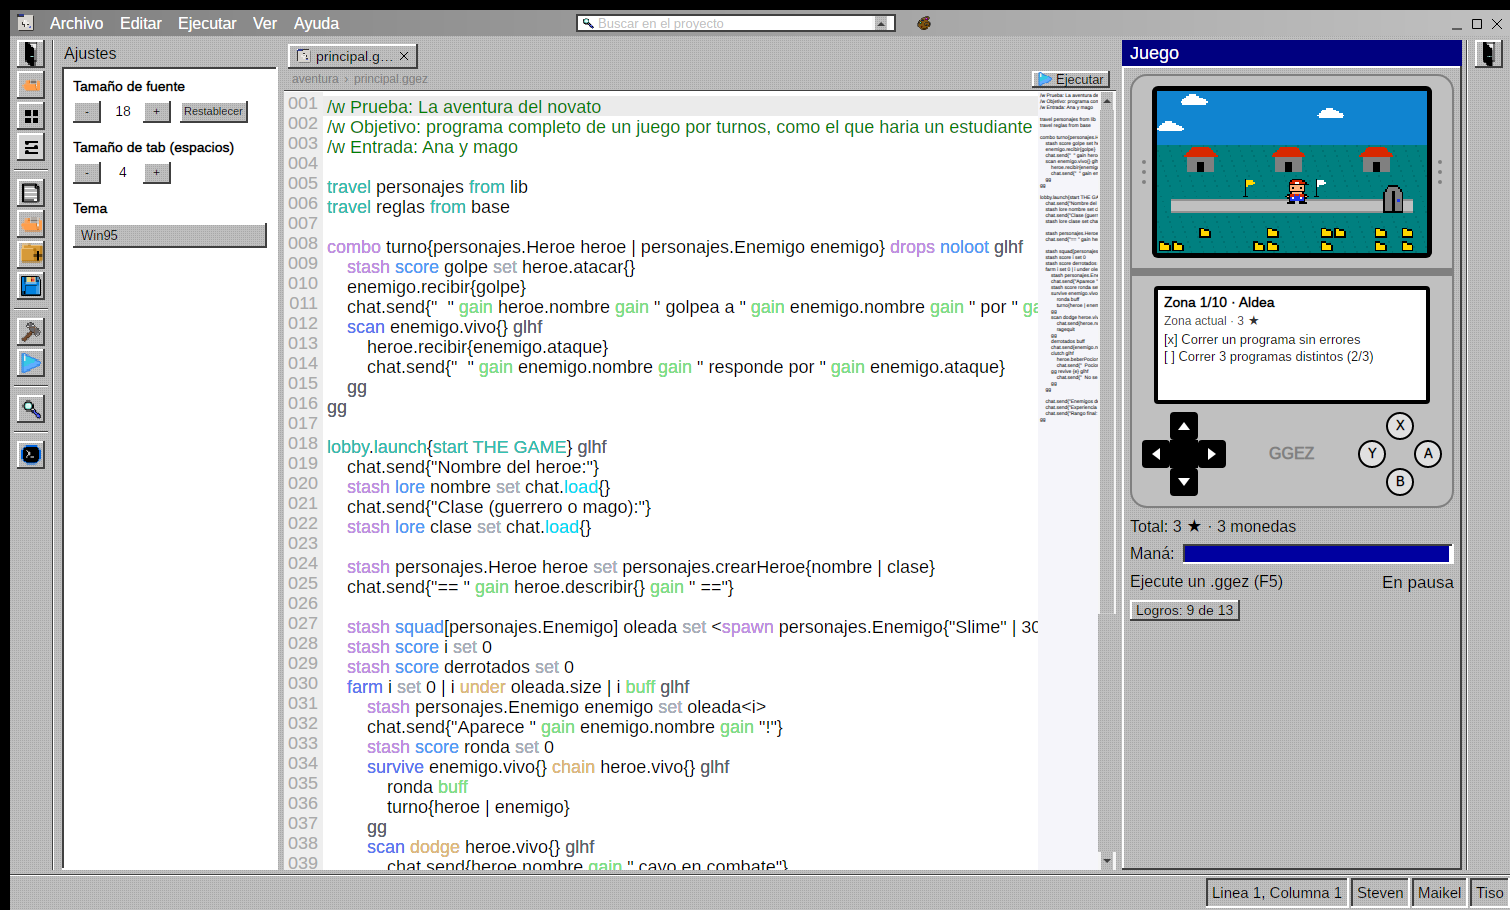
\includegraphics[width=0.92\textwidth]{img/ajustes.png}
\caption{Vista de ajustes.}
\end{figure}

\manualseccion{Ayuda}

\begin{itemize}
  \item \textbf{Ayuda → Sintaxis de GGEZ}: referencia completa del lenguaje, con cada ejemplo junto a su equivalente en Java.
  \item \textbf{Ayuda → Atajos de teclado} (\kw{F1}): lista de todos los atajos.
  \item \textbf{Ayuda → Acerca de}: versión e integrantes.
\end{itemize}

\begin{figure}[H]
\centering
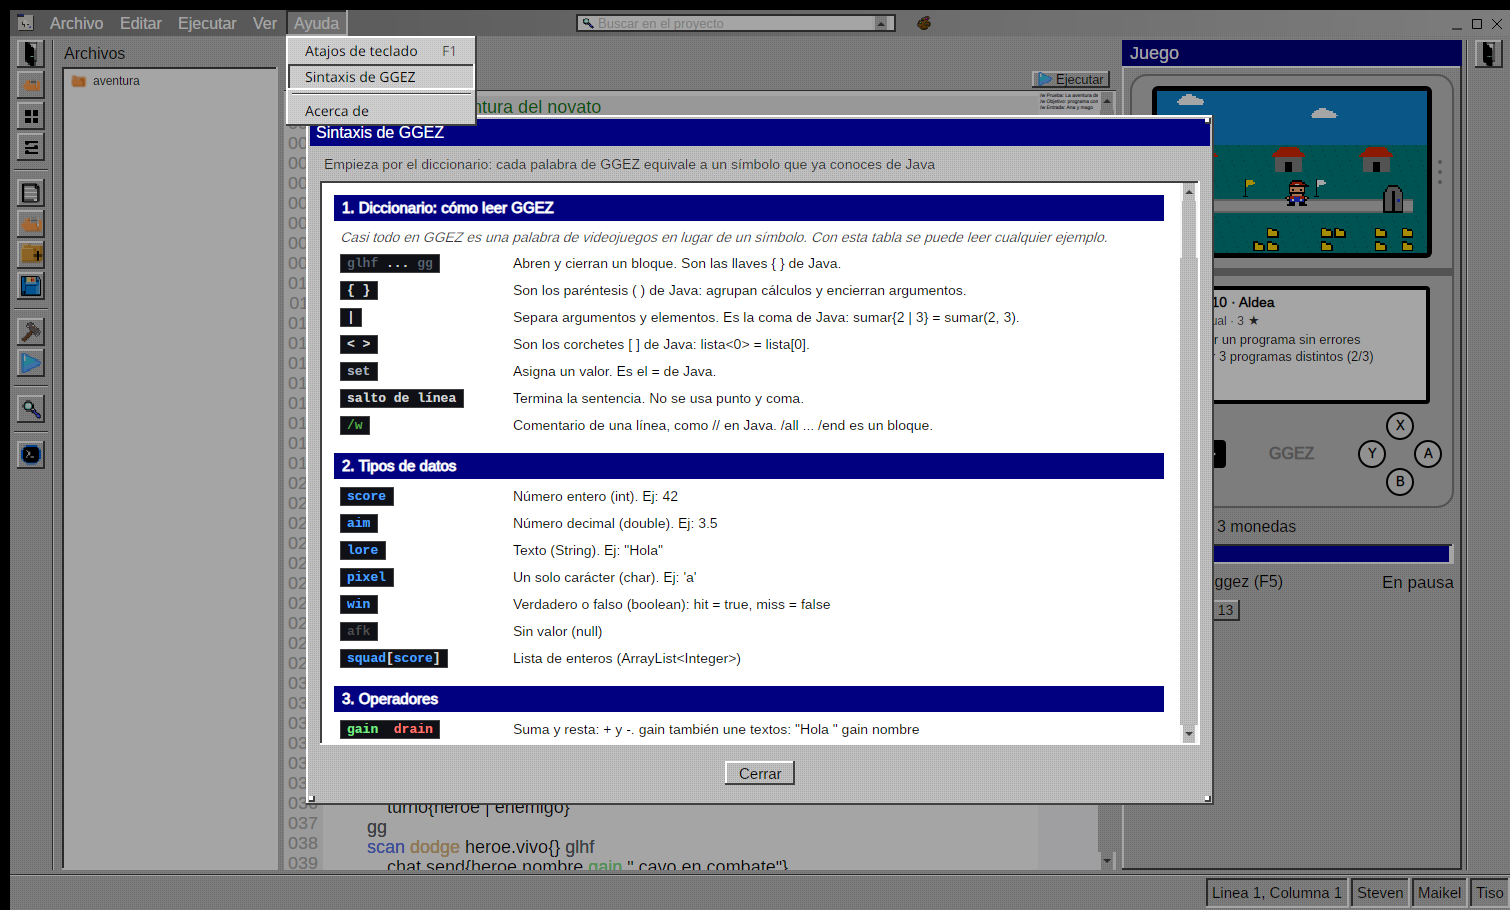
\includegraphics[width=0.92\textwidth]{img/sintaxis.png}
\caption{Referencia del lenguaje con el equivalente en Java.}
\end{figure}

\begin{figure}[H]
\centering
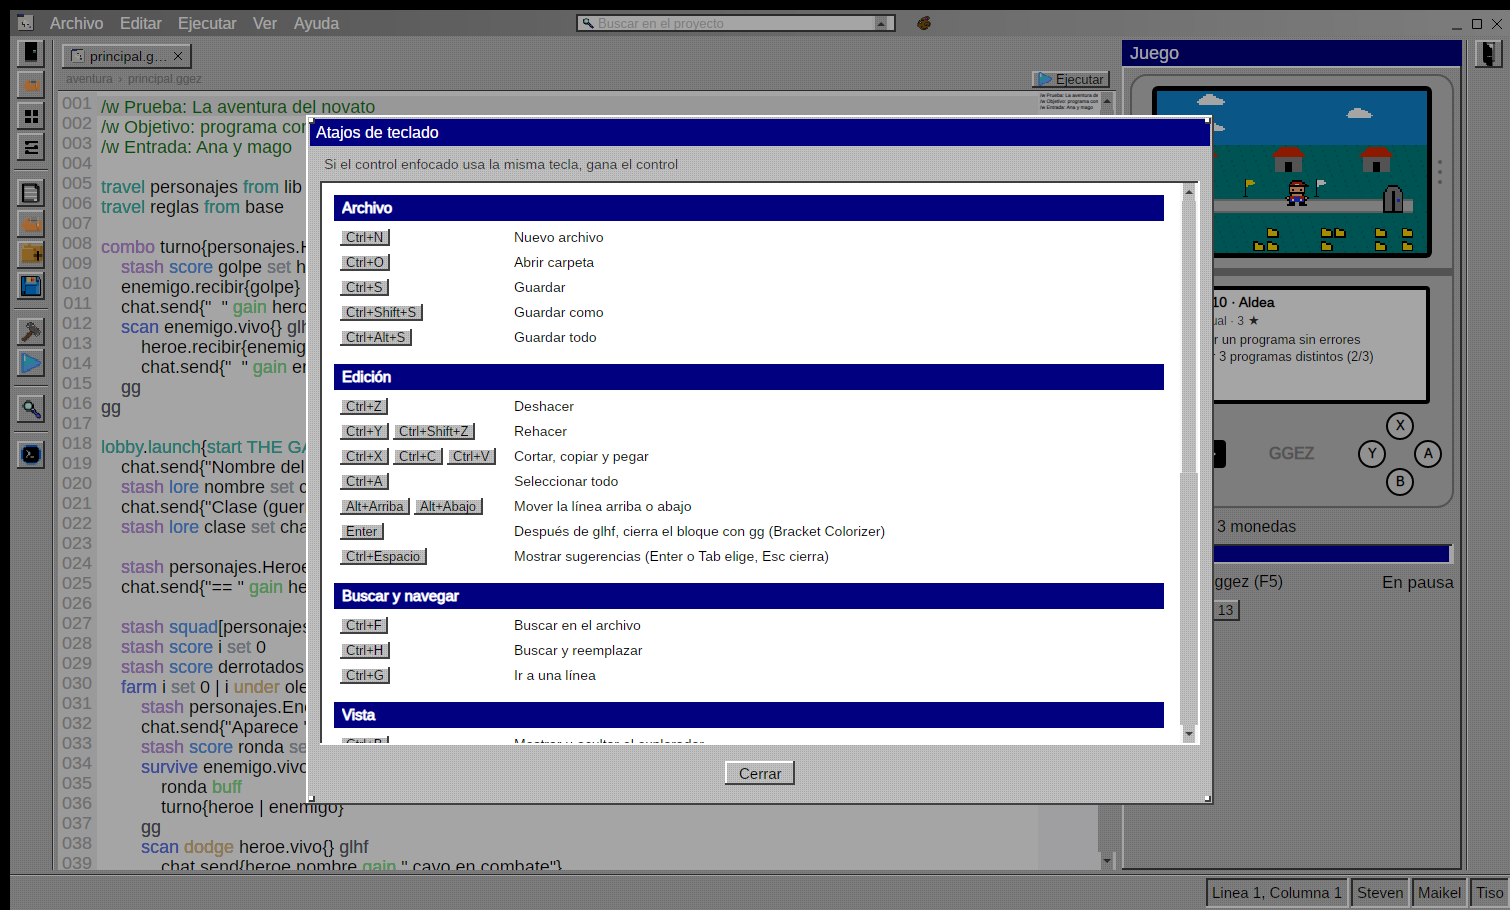
\includegraphics[width=0.92\textwidth]{img/atajos.png}
\caption{Atajos de teclado.}
\end{figure}

\manualseccion{Atajos principales}

\begin{longtable}{|p{5cm}|p{9.4cm}|}\hline
\cab\textbf{Atajo} & \textbf{Acción} \\\hline\endhead
\kw{F5} / \kw{F6} & Ejecutar / Compilar \\\hline
\kw{F1} & Mostrar los atajos \\\hline
\kw{Ctrl+N}, \kw{Ctrl+O} & Nuevo archivo, abrir carpeta \\\hline
\kw{Ctrl+S}, \kw{Ctrl+Alt+S} & Guardar, guardar todo \\\hline
\kw{Ctrl+Z}, \kw{Ctrl+Y} & Deshacer, rehacer \\\hline
\kw{Alt+Arriba} / \kw{Alt+Abajo} & Mover la línea \\\hline
\kw{Ctrl+Espacio} & Sugerencias de autocompletado \\\hline
\kw{Ctrl+F}, \kw{Ctrl+H}, \kw{Ctrl+G} & Buscar, reemplazar, ir a línea \\\hline
\kw{Ctrl+B}, \kw{Ctrl+J} & Mostrar u ocultar explorador y terminal \\\hline
\kw{Ctrl++}, \kw{Ctrl+-}, \kw{Ctrl+0} & Zoom \\\hline
\kw{Ctrl+C} (en la terminal) & Interrumpir el programa \\\hline
\end{longtable}
